\justify
Predecir series temporales con influencias externas no es trivial. Dos familias de modelos han demostrado ser especialmente útiles en ese contexto: los métodos estadísticos de la familia ARIMA —en particular su extensión SARIMAX, que incorpora variables exógenas— y las redes neuronales recurrentes, representadas aquí por las arquitecturas LSTM y GRU. Cada una tiene fortalezas distintas y limitaciones propias; entender su funcionamiento es indispensable para interpretar los resultados del capítulo siguiente.

\justify
SARIMAX parte de un supuesto de linealidad y requiere que la serie sea estacionaria, lo que implica pasos de preprocesamiento explícitos (diferenciación, pruebas de raíz unitaria). Su ventaja es la interpretabilidad: los coeficientes tienen significado estadístico directo. LSTM y GRU, en cambio, aprenden representaciones no lineales de forma automática, a costa de una mayor demanda computacional y menor transparencia en la interpretación de sus parámetros internos.

\justify
Las secciones que siguen presentan la formulación matemática de cada enfoque. El lector familiarizado con series temporales puede ir directamente a la sección que le interese; quien se acerque por primera vez encontrará aquí los conceptos necesarios para seguir el resto del trabajo.

\section{Modelos Estadísticos}
\justify
Para comprender el funcionamiento del modelo SARIMAX (Seasonal AutoRegressive Integrated Moving Average with eXogenous regressors), es necesario primero revisar sus antecedentes conceptuales: los modelos ARIMA y SARIMA.

\subsection{ARIMA}
\justify
El modelo ARIMA (AutoRegressive Integrated Moving Average) es una técnica estadística ampliamente utilizada para el análisis y pronóstico de series temporales. Se clasifica como un modelo lineal, ya que los valores futuros se expresan como combinaciones lineales de observaciones pasadas y de errores previos. \cite{newbold1983arima,lee2011short}
\justify
ARIMA combina tres componentes principales:
 
\begin{itemize}
\item AR (autoregresivo, $p$): supone que la variable $Y_t$ depende linealmente de sus valores anteriores. Por ejemplo, un modelo AR de orden $p$ se define como:
\begin{equation}
 Y_t = \phi_1 Y_{t-1} + \phi_2 Y_{t-2} + \dots + \phi_p Y_{t-p} + \varepsilon_t
\end{equation}
 donde $\varepsilon_t$ es ruido blanco y $\phi_i$ son los coeficientes autoregresivos.

\item I (integrado, $d$): captura la no estacionariedad de la serie mediante diferencias sucesivas. La diferenciación de orden $d$ se expresa como:
\begin{equation}
 \nabla^d Y_t = (1-B)^d Y_t
\end{equation}
 donde $B$ es el operador de rezago $(B Y_t = Y_{t-1})$ y $\nabla^d Y_t$ se utiliza para estabilizar la media y la varianza de la serie.

\item MA (media móvil, $q$): modela la dependencia de la variable con los errores pasados. Un modelo MA de orden $q$ se define como:
\begin{equation}
 Y_t = \varepsilon_t + \theta_1 \varepsilon_{t-1} + \dots + \theta_q \varepsilon_{t-q}
\end{equation}
 donde $\theta_j$ son los coeficientes de la media móvil.

\end{itemize}

\justify
De manera compacta, un ARIMA(p,d,q) se representa como:
\begin{equation}
 (1 - \phi_1 B - \dots - \phi_p B^p)(1 - B)^d Y_t = (1 + \theta_1 B + \dots + \theta_q B^q) \varepsilon_t
\end{equation}

\subsection{SARIMA}
\justify
El modelo SARIMA (Seasonal AutoRegressive Integrated Moving Average), también conocido como modelo ARIMA estacional, es una extensión del enfoque Box–Jenkins, diseñada para capturar patrones estacionales o periódicos en las series temporales.\cite{vagropoulos2016comparison}

\justify
Mientras que el modelo $ARIMA(p, d, q)$ aborda las relaciones no estacionales —tendencias y dependencias de corto plazo—, el modelo $SARIMA(p, d, q)(P, D, Q)_s$ incorpora componentes adicionales que permiten representar comportamientos repetitivos a intervalos regulares, como meses, trimestres o años.

\justify
Los parámetros del modelo tienen la siguiente interpretación:

\begin{itemize}
\item $p$: orden del componente autoregresivo (AR) no estacional, que mide la influencia de valores pasados sobre el actual.
\item $d$: número de diferencias no estacionales necesarias para lograr estacionariedad en la serie.
\item $q$: orden del componente media móvil (MA) no estacional, que modela la dependencia respecto a errores pasados.
\item $P$: orden del componente autoregresivo estacional (SAR).
\item $D$: número de diferencias estacionales aplicadas para eliminar la tendencia o estacionalidad.
\item $Q$: orden del componente media móvil estacional (SMA).
\item $s$: longitud del ciclo estacional (por ejemplo, $s = 12$ para datos mensuales o $s = 4$ para datos trimestrales).

\end{itemize}

\justify
La formulación general del modelo se expresa como:
\begin{equation}
 \Phi_P(B^s)\,\phi_p(B)\,(1 - B)^d\,(1 - B^s)^D\,Y_t
 = \Theta_Q(B^s)\,\theta_q(B)\,\varepsilon_t
\end{equation}

\justify
donde:
\begin{itemize}
\item  $B$ es el operador de rezago $(B Y_t = Y_{t-1})$,

\item  $\phi_p(B)$ y $\theta_q(B)$ son los polinomios no estacionales de los componentes AR y MA,

\item  $\Phi_P(B^s)$ y $\Theta_Q(B^s)$ son los polinomios estacionales de los componentes SAR y SMA, y

\item  $\varepsilon_t$ representa un proceso de ruido blanco.
\end{itemize}

\subsection{SARIMAX}
\justify
El modelo SARIMAX (Seasonal AutoRegressive Integrated Moving Average with eXogenous regressors) constituye una extensión del modelo SARIMA, al incorporar variables exógenas que permiten capturar la influencia de factores externos sobre la variable objetivo. Esta característica lo convierte en un modelo multivariado capaz de representar tanto la estructura temporal interna de la serie como los efectos de variables adicionales que afectan su comportamiento. 
Matemáticamente, el modelo puede expresarse como:

\begin{equation}
 \Phi_P(B^s)\,\phi_p(B)\,(1 - B)^d\,(1 - B^s)^D\,Y_t
 = \beta X_t + \Theta_Q(B^s)\,\theta_q(B)\,\varepsilon_t
\end{equation}

\justify
donde:
\begin{itemize}
\item $Y_t$: variable dependiente o serie temporal a modelar.
\item $X_t$: vector de variables exógenas observadas en el tiempo $t$.
\item $\beta$: vector de coeficientes asociados a las variables exógenas.
\item $B$: operador de rezago $(B Y_t = Y_{t-1})$.
\item $\phi_p(B)$ y $\theta_q(B)$: polinomios no estacionales de los componentes autoregresivo (AR) y de media móvil (MA), respectivamente.
\item $\Phi_P(B^s)$ y $\Theta_Q(B^s)$: polinomios estacionales de los componentes autoregresivo (SAR) y de media móvil (SMA).
\item $d$: número de diferencias no estacionales necesarias para eliminar la tendencia.
\item $D$: número de diferencias estacionales necesarias para eliminar la periodicidad.
\item $s$: longitud del ciclo estacional.
\item $\varepsilon_t$: término de error aleatorio o ruido blanco, $\varepsilon_t \sim N(0, \sigma^2)$.
\end{itemize}

\section{Machine Learning}
\justify
Una definición concisa de Machine Learning (ML) es la de Murphy \cite{murphy2012machine}: métodos capaces de identificar patrones en los datos de manera automática y usar esos patrones para predecir o decidir bajo incertidumbre. Lo que hace interesante a esta definición es que el énfasis está en \textit{aprender de los datos}, no en seguir reglas codificadas por un experto.

\justify
Dentro del ML, el aprendizaje profundo (Deep Learning, DL) ocupa un lugar particular. Es, en esencia, una subrama que trabaja con redes neuronales de múltiples capas, capaces de representar relaciones muy complejas sin que el investigador tenga que definirlas explícitamente \cite{chollet2021deep}. La diferencia práctica es relevante: mientras un modelo de ML clásico suele requerir que el analista seleccione y construya las características más informativas, un modelo de DL puede derivarlas directamente de los datos crudos. Esa autonomía tiene un costo — más datos, más cómputo, menos interpretabilidad — pero en series temporales complejas y no lineales, como las de precios de materiales de construcción, esa capacidad de abstracción resulta valiosa.

\justify
El ML puede clasificarse en 3 categorías principales:

\begin{itemize}
\item Aprendizaje supervisado: es un enfoque del ML en el cual el modelo se entrena utilizando un conjunto de datos etiquetado, es decir, donde las entradas están asociadas con sus salidas correspondientes. Durante el proceso de entrenamiento, el algoritmo aprende a relacionar las variables de entrada con las salidas esperadas, con el objetivo de generalizar ese conocimiento a nuevos datos. Uno de los problemas más comunes dentro del aprendizaje supervisado es la clasificación \cite{allix2003epistemology}.

\item Aprendizaje no supervisado: se caracteriza porque los datos de entrenamiento no poseen etiquetas o salidas conocidas. En este enfoque, el modelo busca descubrir patrones o estructuras ocultas dentro del conjunto de datos sin intervención externa. Las técnicas más comunes incluyen clustering, fuzzy clustering, clustering jerárquico, K-means y association rule mining \cite{mathur1999socialization}. En estos casos, los algoritmos agrupan los datos en función de su similitud, permitiendo desarrollar marcos de análisis basados en la información observada.

\item Aprendizaje por refuerzo: es un enfoque en el que un agente, generalmente representado por un programa informático, interactúa con un entorno dinámico con el objetivo de alcanzar una meta específica. A medida que ejecuta acciones, el agente recibe retroalimentación en forma de recompensas o penalizaciones, lo que le permite aprender una política óptima que maximiza la recompensa acumulada a lo largo del tiempo \cite{kaelbling1996reinforcement}.
\end{itemize}

\section{Artificial Neural Networks (ANN)}
\justify
Una Red Neuronal Artificial (ANN) es un modelo computacional inspirado en la estructura y funcionamiento del sistema nervioso biológico, especialmente en la forma en que las neuronas procesan y transmiten información. Está compuesta por unidades llamadas neuronas artificiales, organizadas en capas y conectadas mediante pesos sinápticos, que determinan la influencia de una neurona sobre otra \cite{martinez2014metodologia}.
\justify
Cada conexión entre neuronas posee un peso que refleja la importancia de la señal transmitida. Durante el proceso de entrenamiento, los pesos se modifican iterativamente mediante algoritmos de optimización, con el fin de minimizar la diferencia entre la salida real y la deseada.
\justify
De esta forma, las ANNs reproducen el comportamiento de sistemas complejos, permitiendo modelar relaciones no lineales entre variables de entrada y salida. Su capacidad de procesar información en paralelo y en tiempo real constituye una de sus principales ventajas, favoreciendo su uso en clasificación y reconocimiento de patrones en sistemas de alta complejidad. La capacidad fundamental de las ANNs radica en su habilidad para identificar no linealidades en series temporales, siendo por ello ampliamente aplicadas en la predicción de fenómenos económicos y financieros \cite{villada2016redes}.
\justify
Las neuronas artificiales se estructuran en capas jerárquicas, clasificadas en tres tipos: capa de entrada, capas ocultas y capa de salida.
La capa de entrada recibe los datos del entorno; las capas ocultas procesan la información y extraen patrones complejos, siendo su número y tamaño variables según el problema; finalmente, la capa de salida produce la respuesta del modelo, adaptada al tipo de tarea (una neurona para regresión o varias para clasificación).
El flujo de información se produce de forma secuencial desde la entrada hasta la salida, donde cada neurona transmite su salida como entrada a las neuronas de la capa siguiente.
La Figura \ref{fig:rna} muestra la estructura general que presenta una red neuronal.

\begin{figure}[H]
    \centering
    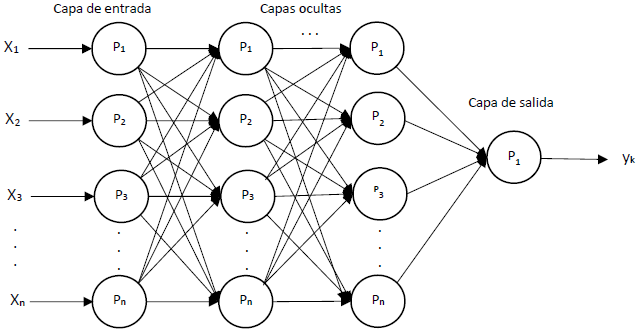
\includegraphics[width=0.8\textwidth]{images/rna.png}
    \caption{Estructura general de una Red Neuronal Artificial}
    \label{fig:rna}
\end{figure}

\justify
Una ANN está compuesta por nodos llamados neuronas, que se conectan entre sí mediante enlaces denominados \textit{sinapsis}. Estas conexiones determinan cómo se transmite la información y, en conjunto, definen el comportamiento de la red. En la Figura~\ref{fig:rna} se observa un ejemplo con dos capas ocultas, donde $X_n$ representan las variables de entrada, $y_n$ las salidas y $\varphi$ la función de activación.
\justify
Cada neurona se conecta con otras a través de sinapsis cuyo peso, representado por $W_{ji}$, refleja la fuerza o importancia de la conexión. La Ecuación~\ref{eq:neurona_salida} expresa matemáticamente cómo se calcula la salida de una neurona: las entradas $x_n$ son ponderadas por los pesos $W_{ji}$ y transformadas mediante la función de activación $\varphi$. Además, cada neurona posee un valor umbral que ajusta su nivel de respuesta.

\begin{equation}
    y_{i} = \varphi \left( \sum_{i=0}^{n} W_{ji}x_{i} \right)
    \label{eq:neurona_salida}
\end{equation}

\subsection{Recurrent Neural Network (RNN)}
\justify
Las Redes Neuronales Recurrentes (RNN) surgieron en la década de 1980, aunque su aplicación práctica se ha expandido recientemente gracias al incremento del poder computacional proporcionado por las unidades de procesamiento gráfico. Estas redes resultan especialmente útiles para el tratamiento de datos secuenciales, ya que cada neurona o unidad posee una memoria interna que le permite retener información sobre las entradas previas. A diferencia de las redes neuronales tradicionales, las RNN incorporan bucles de retroalimentación que permiten transferir información entre neuronas mientras se procesan las secuencias de entrada \cite{lazzeri2020machine}.
\justify
Las RNNs son un tipo de red que mantiene información de pasos anteriores mediante bucles internos y estados ocultos, lo que les permite recordar y aprovechar el contexto pasado. 
Mientras que las redes tradicionales aprenden únicamente de los datos actuales, las RNNs integran el estado oculto como una forma de memoria que se actualiza con cada nueva entrada.
Esta memoria, almacenada en un vector, se combina con el nuevo dato de entrada para producir una salida (Y) y actualizar el estado interno, como se muestra en la Figura \ref{fig:rnn}.

\begin{figure}[H]
    \centering
    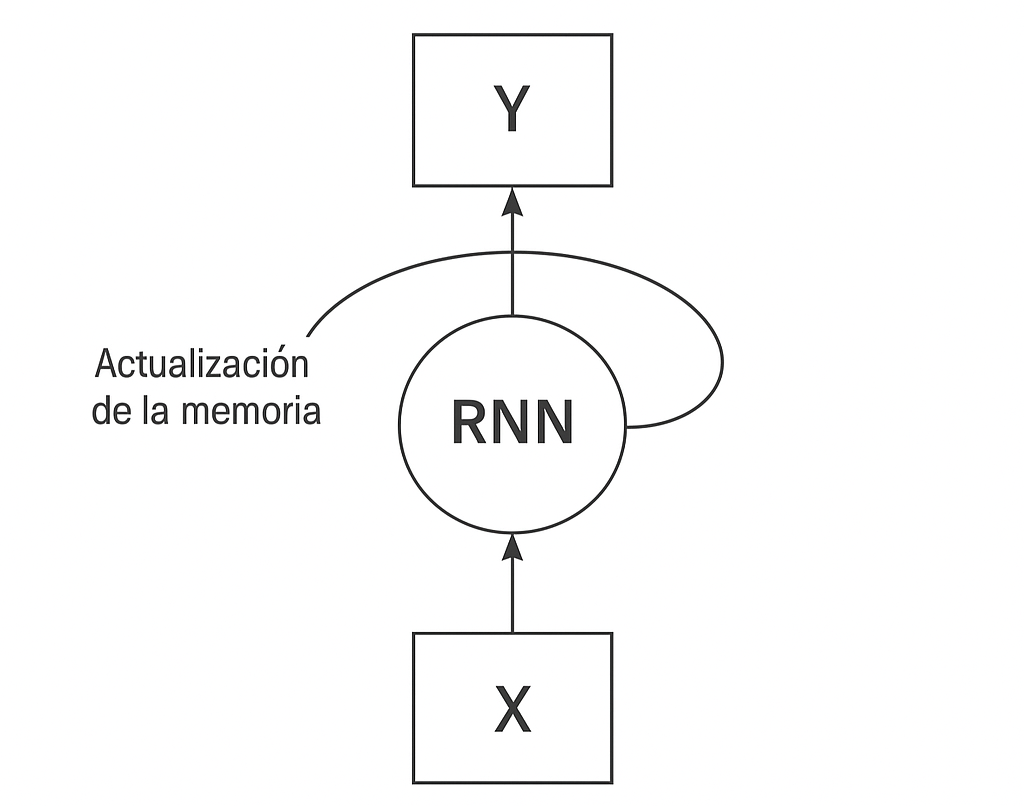
\includegraphics[width=0.4\textwidth]{images/rnn.png}
    \caption{Estructura de una Red Neuronal Recurrente (RNN)}
    \label{fig:rnn}
\end{figure}

\justify
Las unidades de una RNN se denominan \textit{unidades recurrentes} porque el valor actual depende de manera recurrente de los eventos previos. Este comportamiento puede interpretarse como la existencia de múltiples copias del mismo nodo, cada una transmitiendo información de forma secuencial hacia su sucesor. Esta relación recursiva se ilustra en la Figura~\ref{fig:rnn_arc}.

\begin{figure}[H]
    \centering
    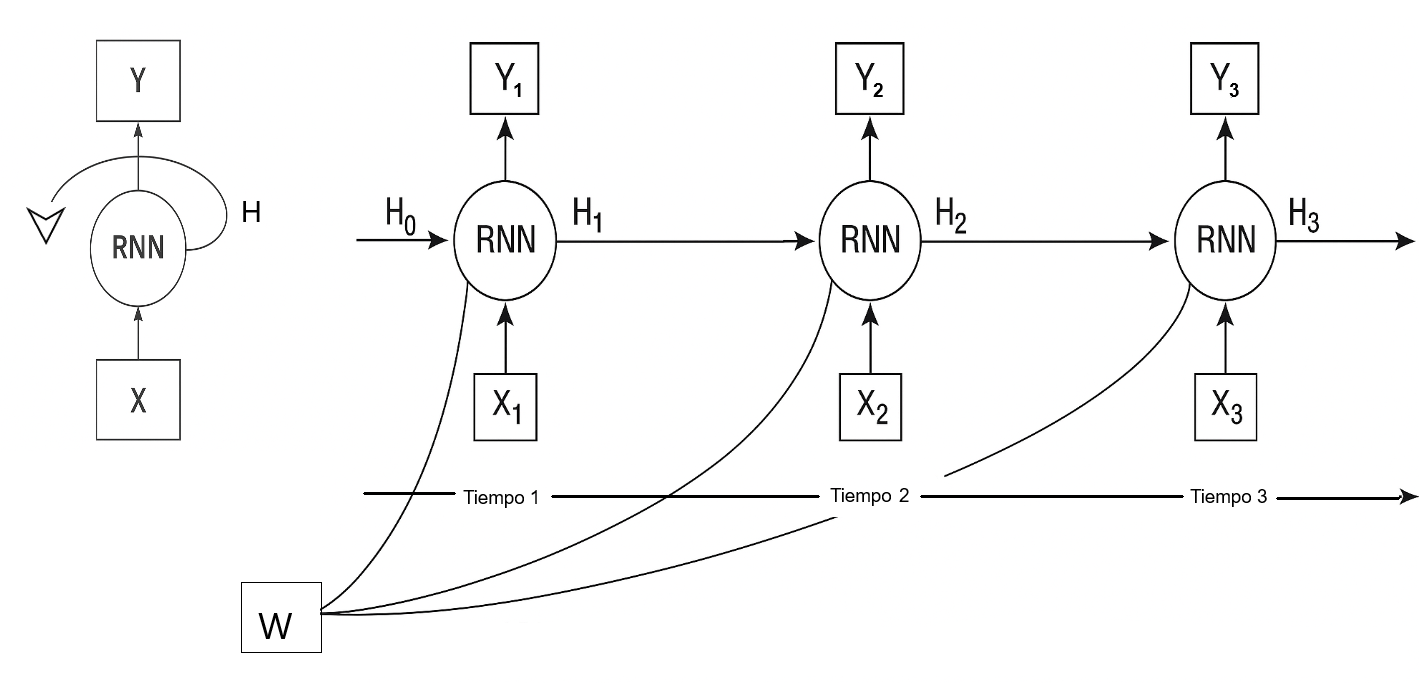
\includegraphics[width=0.6\textwidth]{images/rnn_arc.png}
    \caption{Arquitectura de una Red Neuronal Recurrente (RNN)}
    \label{fig:rnn_arc}
\end{figure}

\justify
En la Figura~\ref{fig:rnn_arc} se representa la arquitectura de una RNN. Este tipo de red posee un estado interno oculto, denotado como $H$, que puede retroalimentarse dentro de la propia red. La RNN procesa los valores de entrada $X$ y genera valores de salida $Y$. El estado oculto $H$ permite que la información se propague de un nodo a otro dentro de la red, organizándose en secuencias o vectores que contienen información tanto de la entrada actual como de las anteriores. Posteriormente, dicho vector pasa por la función de activación tangente hiperbólica ($\tanh$), que regula los valores dentro del rango $[-1,1]$.

\justify
Cada unidad cuenta con tres conjuntos de pesos: uno para las entradas ($X$), otro para los estados ocultos previos ($H$) y otro para las salidas ($Y$). Estos pesos se ajustan durante el proceso de entrenamiento mediante el método de descenso del gradiente, el cual actualiza los parámetros minimizando una función de pérdida. 

\subsection{Long Short-Term Memory (LSTM)}
\justify
Las redes LSTM, introducidas por Hochreiter y Schmidhuber \cite{hochreiter1997long}, constituyen una variante de las RNNs desarrollada con el propósito de superar las limitaciones de estas últimas al aprender dependencias de largo plazo en secuencias.
En los modelos RNN convencionales, la información se transmite a través de los estados ocultos a lo largo del tiempo, pero durante el proceso de entrenamiento basado en retropropagación a través del tiempo (BPTT) los gradientes tienden a desvanecerse o explotar.
Este fenómeno impide que las RNN aprendan eficazmente relaciones entre eventos temporalmente distantes.
\justify
El modelo LSTM introduce una unidad de memoria interna, denominada celda, que puede mantener información constante a lo largo de múltiples pasos temporales, resolviendo de manera efectiva el problema del desvanecimiento del gradiente.
Cada celda incluye un estado interno $C_t$ y un estado oculto $H_t$, junto con un conjunto de compuertas multiplicativas que regulan el flujo de información.
\justify
El principio clave es que el estado interno posee una autoconexión de peso fijo igual a 1, lo cual garantiza que los gradientes puedan fluir a través del tiempo sin desaparecer, manteniendo la información relevante.
\subsubsection{Compuertas del LSTM}
\justify
Cada celda LSTM cuenta con tres compuertas principales: entrada, olvido y salida.
\justify
Estas compuertas controlan de manera diferenciada cómo se actualiza y utiliza la información almacenada en la celda:

\begin{itemize}
\item Puerta de entrada $I_t$: regula cuánta información nueva proveniente de la entrada actual $X_t$ se incorpora al estado interno.
\item  Puerta de olvido $F_t$: decide qué fracción del estado anterior $C_{t-1}$ se conserva o se descarta.
\item  Puerta de salida $O_t$: determina cuánto del estado interno actualizado influirá en la salida del modelo $H_t$.
\end{itemize}

\justify
Cada una de estas compuertas se calcula mediante una capa completamente conectada seguida de una función sigmoide, que restringe los valores al intervalo (0, 1). Matemáticamente, para un conjunto de $n$ observaciones y $h$ unidades ocultas, las compuertas se definen como:

\begin{equation}
I_t = \sigma(X_t W_{xi} + H_{t-1} W_{hi} + b_i) \
\end{equation}

\begin{equation}
F_t = \sigma(X_t W_{xf} + H_{t-1} W_{hf} + b_f) \
\end{equation}

\begin{equation}
O_t = \sigma(X_t W_{xo} + H_{t-1} W_{ho} + b_o)
\end{equation}

\justify
donde $W_{xi}, W_{xf}, W_{xo} \in \mathbb{R}^{d \times h}$ y $W_{hi}, W_{hf}, W_{ho} \in \mathbb{R}^{h \times h}$ son las matrices de pesos asociados a la entrada y al estado oculto previo respectivamente, mientras que $b_{i}, b_{f}, b_{o} \in \mathbb{R}^{1 \times h}$ representa los sesgos.

\subsubsection{Estado candidato y actualización del estado interno}
\justify
Además de las compuertas, la celda genera un estado candidato $\tilde{C}_t$, que representa la nueva información potencial a incorporar al estado interno.
Este se obtiene aplicando una activación tangente hiperbólica $(\tanh)$ sobre una combinación lineal de la entrada y el estado oculto previo:

\begin{equation}
\tilde{C}_t = \tanh(X_t W_{xc} + H_{t-1} W_{hc} + b_c)
\end{equation}

\justify
Posteriormente, el estado interno de la celda $C_t$ se actualiza combinando la información retenida y la información nueva de acuerdo con:

\begin{equation}
C_t = F_t \odot C_{t-1} + I_t \odot \tilde{C}_t
\end{equation}

\justify
donde $\odot$ representa el producto elemento a elemento (Hadamard).
\justify
En este esquema, la puerta de olvido controla cuánto del estado anterior se preserva, mientras que la puerta de entrada modula cuánto de la nueva información se añade.
Si $F_t = 1$ y $I_t = 0$, la celda retiene íntegramente la información anterior, actuando como una memoria persistente.

\subsubsection{Generación del estado oculto}
\justify
El estado oculto de salida $H_t$ es la señal que se propaga a las capas siguientes o al paso temporal siguiente dentro de la secuencia.
\justify
Se obtiene aplicando una función tangente hiperbólica al estado interno actualizado y modulando el resultado mediante la puerta de salida:

\begin{equation}
H_t = O_t \odot \tanh(C_t)
\end{equation}

\justify
Este mecanismo permite que el modelo decida en qué momentos la información almacenada en la celda debe influir en la salida, y en qué momentos debe permanecer “oculta”, manteniendo la información sin propagarla.
\justify
La Figura \ref{fig:lstmcell} ilustra la estructura interna de una celda de memoria LSTM. En ella se observa cómo las compuertas de entrada $I_t$, olvido $F_t$ y salida $O_t$ regulan el flujo de información a través del estado interno de la celda $C_t$.
\justify
La compuerta de entrada controla cuánta información nueva proveniente de la entrada $X_t$ se incorpora, mientras que la compuerta de olvido determina qué parte del estado previo $C_{t-1}$ debe descartarse. Finalmente, la compuerta de salida define qué proporción del estado interno actualizado influye en la salida del modelo $H_t$.

\begin{figure}[H]
    \centering
    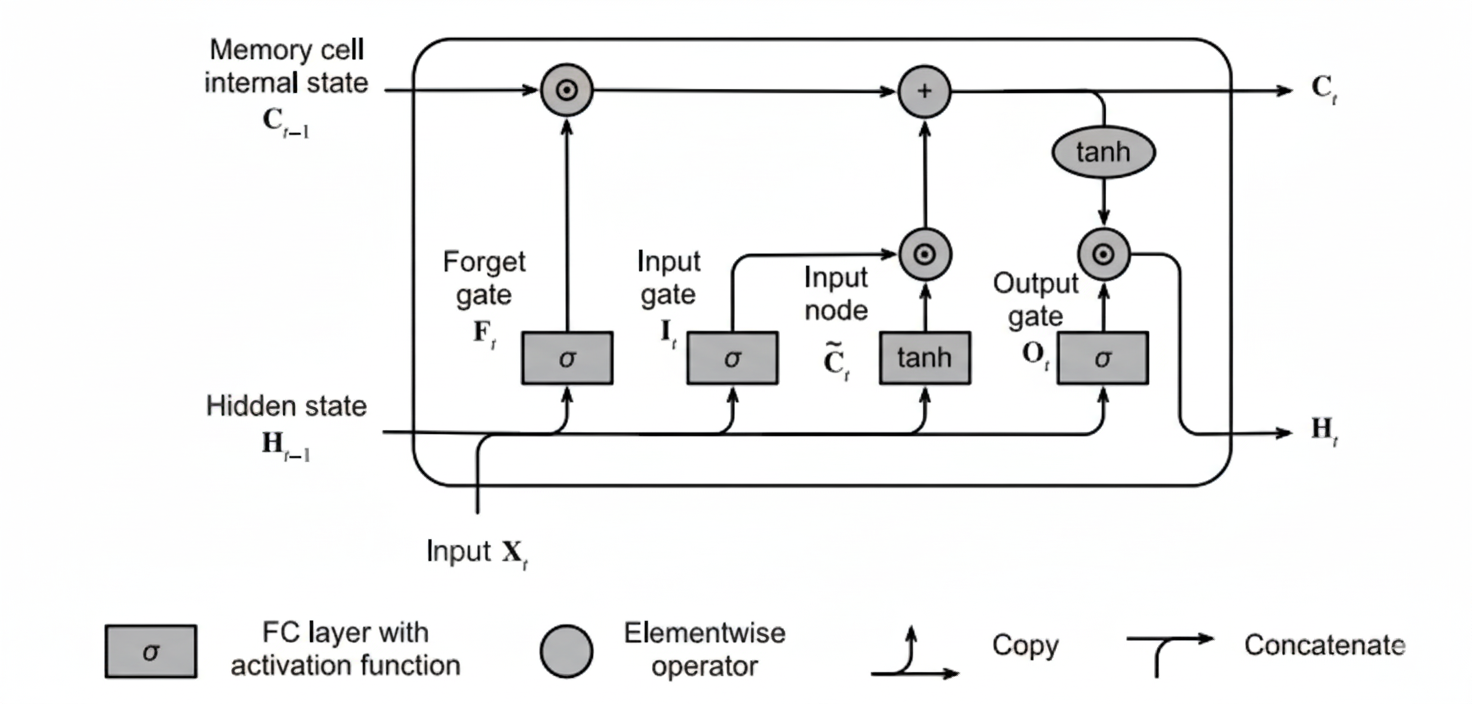
\includegraphics[width=0.8\textwidth]{images/lstm_cell.png}
    \caption{Estructura interna de una celda de memoria LSTM.} 
    \label{fig:lstmcell}
\end{figure}

\subsection{Gated Recurrent Unit (GRU)}
\justify
Las redes GRU fueron introducidas por Cho et al. \cite{cho2014learning} como una simplificación del modelo LSTM. El objetivo fue conservar la capacidad de las redes recurrentes para modelar dependencias a largo plazo, reduciendo al mismo tiempo la complejidad computacional y el número de parámetros.
\justify
A diferencia de las LSTM, las GRU fusionan el estado de la celda y el estado oculto en una única representación, lo que las hace más eficientes sin sacrificar desempeño en la mayoría de los problemas de predicción secuencial.
\subsubsection{Estructura general}
\justify
La arquitectura GRU incorpora dos compuertas principales:
\begin{itemize}
\item Compuerta de reinicio (reset gate), que controla cuánta información del estado previo debe olvidarse.
\item Compuerta de actualización (update gate), que determina en qué medida se conserva la información anterior o se actualiza con la nueva entrada.
\end{itemize}
\justify
Ambas compuertas se activan mediante funciones sigmoides, lo que restringe sus valores al rango (0, 1).

\subsubsection{Compuertas de reinicio y actualización}
\justify
Sea $X_t \in \mathbb{R}^{n \times d}$ el vector de entrada en el instante $t$, donde $n$ representa el tamaño del lote y $d$ la dimensión de las variables de entrada.
\justify
Sea además $H_{t-1} \in \mathbb{R}^{n \times h}$ el estado oculto proveniente del paso temporal anterior, con $h$ unidades ocultas.
\justify
La compuerta de reinicio $R_t \in \mathbb{R}^{n \times h}$ y la compuerta de actualización $Z_t \in \mathbb{R}^{n \times h}$ se calculan como:

\begin{equation}
R_t = \sigma(X_t W_{xr} + H_{t-1} W_{hr} + b_r)
\end{equation}

\begin{equation}
Z_t = \sigma(X_t W_{xz} + H_{t-1} W_{hz} + b_z)
\end{equation}

\justify
donde $W_{xr}, W_{xz} \in \mathbb{R}^{d \times h}$ y $W_{hr}, W_{hz} \in \mathbb{R}^{h \times h}$ son matrices de pesos, mientras que $b_r, b_z \in \mathbb{R}^{1 \times h}$ son los términos de sesgo (\textit{bias}).
\justify
Las funciones sigmoides $\sigma(\cdot)$ garantizan que cada componente de las compuertas adopte valores entre 0 y 1, controlando el grado de influencia de la información anterior y la nueva.

\justify
Intuitivamente:
\begin{itemize}
\item Cuando $R_t$ toma valores cercanos a 0, la red tiende a olvidar información previa, reiniciando parte del estado.
\item Cuando $Z_t$ se aproxima a 1, la red adopta el nuevo estado candidato, actualizando la información con la entrada actual.
\end{itemize}

\subsubsection{Estado oculto candidato}

\justify
La compuerta de reinicio regula la combinación entre la información previa y la nueva entrada.
\justify
Integrando este comportamiento, se define un estado oculto candidato $\tilde{H}_t \in \mathbb{R}^{n \times h}$ como:

\begin{equation}
\tilde{H}_t = \tanh(X_t W_{xh} + (R_t \odot H_{t-1}) W_{hh} + b_h)
\end{equation}

\justify
donde $W_{xh} \in \mathbb{R}^{d \times h}$ y $W_{hh} \in \mathbb{R}^{h \times h}$ son matrices de pesos, $b_h \in \mathbb{R}^{1 \times h}$ son los términos de sesgo (\textit{bias}), el símbolo $\odot$ indica el producto de Hadamard, es decir, una multiplicación elemento a elemento, y la función de activación $\tanh$ limita los valores del estado candidato al intervalo $(-1,1)$.

\justify
En este paso, la compuerta $R_t$ decide cuánto del estado oculto previo $H_{t-1}$ debe combinarse con la nueva información $X_t$.
Si $R_t$ es cercano a cero, el modelo tiende a ignorar el pasado, comportándose como una red neuronal multicapa convencional.
Por el contrario, si $R_t$ es cercano a uno, el modelo retiene información previa, asemejándose a un RNN estándar.

\subsubsection{Actualización del estado oculto}
\justify
Finalmente, la compuerta de actualización $Z_t$ controla el equilibrio entre el estado anterior y el nuevo candidato.
\justify
El estado oculto final $H_t$ se calcula como:

\begin{equation}
H_t = (1 - Z_t) \odot H_{t-1} + Z_t \odot \tilde{H}_t
\end{equation}  

\justify
donde $Z_t$ actúa como un mecanismo de interpolación entre el pasado y el presente.

\begin{itemize}
\item Si $Z_t \approx 1$, el modelo adopta completamente el nuevo estado candidato $\tilde{H}_t$, actualizando la información.
\item Si $Z_t \approx 0$, el modelo mantiene la memoria previa $H_{t-1}$, ignorando la entrada actual.
\end{itemize}

\justify
Este diseño permite a las GRU manejar eficientemente dependencias a corto y largo plazo, ya que:

\begin{itemize}
\item La compuerta de reinicio captura relaciones de corto plazo, al controlar el olvido parcial;
\item La compuerta de actualización permite retener información de largo plazo, al preservar estados relevantes.
\end{itemize}

\justify
La Figura \ref{fig:grucell} representa la estructura interna de una celda GRU. 
A diferencia de la arquitectura LSTM, la GRU combina las funciones de las compuertas de entrada y olvido en una sola compuerta de actualización $Z_t$, y utiliza además una compuerta de reinicio $R_t$ que controla la influencia del estado previo $H_{t-1}$ en el cálculo del nuevo estado candidato $\tilde{H}_t$.

\justify
De esta manera, la GRU logra capturar dependencias temporales a largo plazo con una estructura más simple y menos parámetros que la LSTM.

\begin{figure}[H]
    \centering
    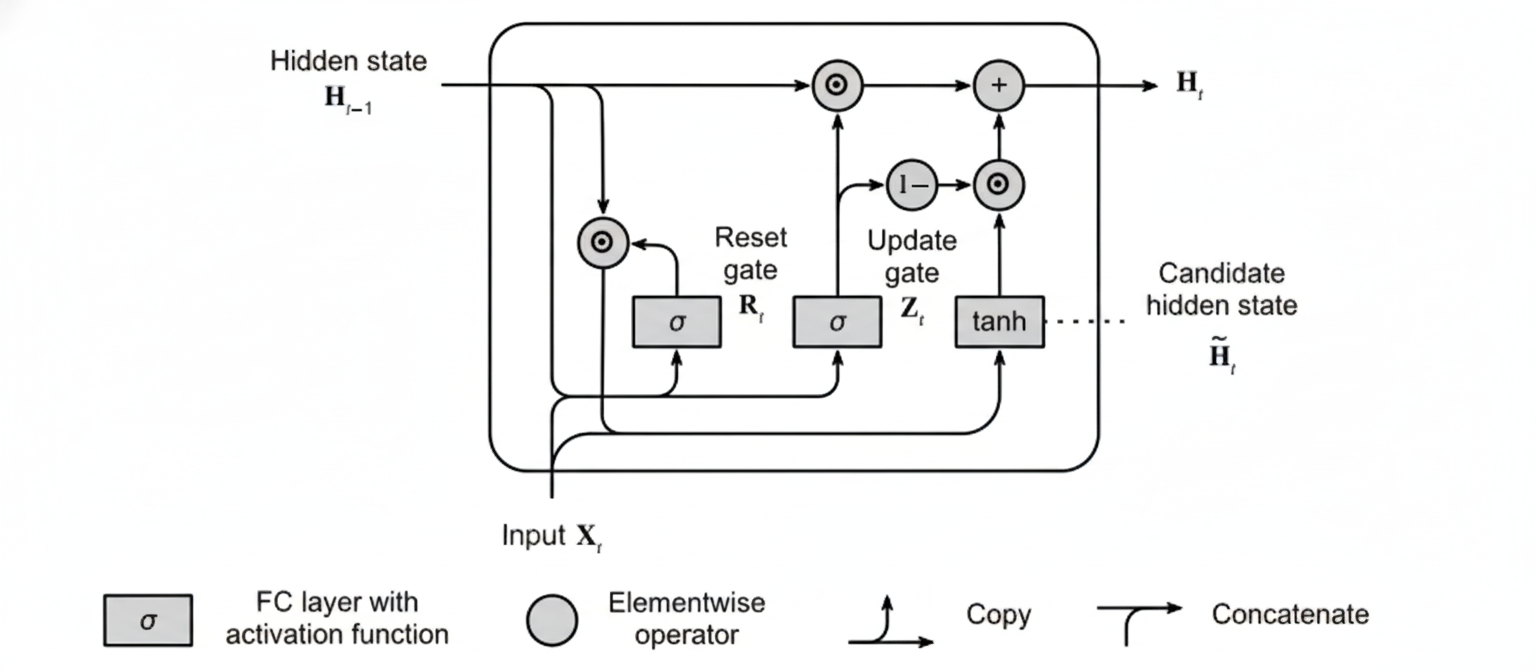
\includegraphics[width=0.8\textwidth]{images/gru_cell.png}
    \caption{Estructura interna de una celda de memoria GRU.}
    \label{fig:grucell}
\end{figure}

\section{Índices de rendimiento}

\justify
Para evaluar el desempeño de un modelo predictivo, se recurre al uso de métricas estadísticas que permiten cuantificar la precisión de las estimaciones realizadas respecto a los valores observados. 

\justify
En este trabajo se emplea como medida principal la \textit{Raíz del Error Medio Cuadrático} (\textit{Root Mean Squared Error} – RMSE), ampliamente utilizada en problemas de predicción y regresión por su capacidad de reflejar la magnitud promedio de los errores de predicción.

\justify
El RMSE evalúa la diferencia promedio entre los valores reales $y_i$ y los valores estimados $\hat{y}_i$ generados por el modelo, penalizando de forma más severa los errores de gran magnitud debido a la elevación al cuadrado de las diferencias. Su formulación matemática se expresa como:

\begin{equation}
    RMSE = \sqrt{\frac{1}{n} \sum_{i=1}^{n} (y_i - \hat{y}_i)^2}
\end{equation}

\justify
donde $n$ representa el número total de observaciones, $y_i$ el valor observado y $\hat{y}_i$ el valor predicho correspondiente. El resultado del RMSE se expresa en las mismas unidades que la variable analizada, lo cual facilita su interpretación directa.

\justify
Un valor de RMSE igual a cero indica un ajuste perfecto entre los valores reales y las predicciones, mientras que valores más elevados reflejan un menor grado de precisión del modelo. En este sentido, el RMSE constituye un indicador robusto para comparar el desempeño de diferentes modelos predictivos, permitiendo identificar aquel que logra minimizar el error medio en las estimaciones.
